\documentclass[conference,a4paper,11pt]{IEEEtran}

\usepackage{xcolor}
\usepackage{listings}

\usepackage[pdftex]{graphicx}
\graphicspath{{./img/}}
\DeclareGraphicsExtensions{.png}

% correct bad hyphenation here
\hyphenation{op-tical net-works semi-conduc-tor}

\definecolor{listing-bg}{gray}{0.96}

\begin{document}
\title{A Service Mesh Built with Jails on FreeBSD}

\author{\IEEEauthorblockN{Esteban Barrios}
\IEEEauthorblockA{trivago N.V.\\
\emph{esteban.barrios@trivago.com}}
\and
\IEEEauthorblockN{Luca Pizzamiglio}
\IEEEauthorblockA{trivago N.V., FreeBSD\\
\emph{pizzamig@FreeBSD.org}}}

\maketitle

\begin{abstract}
Containers have impacted how web services are developed, built and deployed nowadays. In more detail, Docker containers made available a different way of build and deploy services: the container con be build on a system and deployed in many copies on other systems.

FreeBSD is an operating system that provides all the technologies needed to build a container model: \texttt{jail(8)}, \texttt{VNET(9)}, \texttt{zfs(8)}, firewalls like \texttt{pf(4)} or \texttt{ipfw(8)}, \texttt{rctl(4)}. In time, several tools have been developed to help sysadmin to manage jails.

However, the typical jail management process is designed to build the jail directly on the host machine.

The solution we propose aim to split the jail creation and the jail deploy, providing tools to create jail images via \texttt{pot(8)} and deploying them using standard service mesh tools, like consul and nomad.
\end{abstract}

\section{Introduction}\label{sec:Introduction}
In cloud computing, container-orchestration systems are establishing themselves as a de-facto standard solutions to deploy, scale and manage web and micro services; those tools rely on container technologies, mainly Docker~\cite{docker}, to deploy container images, that already includes specific applications. Docker container images can be built on a system and then deployed on other systems. Docker container is a Linux native technology, other operating systems can run Docker container via a Linux kernel running in a virtual machine.

We believed that FreeBSD has all the technologies to replicate such container-based paradigm, even if with minor differencies in the container model definition.

To prove that FreeBSD is a container-ready OS, we decided to implement a container model and to integrate it in a cluster management software, commonly used to orchestrate Docker container on Linux.

In Section~\ref{sec:Background}  we present a brief overview of jails management programs available on FreeBSD.\@

In Section~\ref{sec:pot} we present pot, our container model based on FreeBSD technologies and ways to create images.

In Section~\ref{sec:ServiceMesh} we illustrate the open-source cluster management software we extended to support pot.

In Section~\ref{sec:nomad-pot-driver} we breafily describe how the driver works.

In Section~\ref{sec:Images} we discuss \texttt{pot} images and the current work around the topic.

In Section~\ref{sec:Conclusion}  we present our concusions and future works.
 
\section{Background}\label{sec:Background}
\texttt{jail(8)} is a technology implemented many years ago by \texttt{phk@}~\cite{jail} to improve the isolation capabilities of \texttt{chroot(2)}. Similarly to chroot, jail will changes the root directory for a specific program, but it will also isolate processes, the network traffic and other capabilities can be limited or forbidden, like device access or file system mount.

Over time, several programs have been written to automate some repetitive tasks related to jail management: ezjail, qjail, iocage, CBSD, BastilleBSD.\@

Each of them helps to create and manage jails on FreeBSD, with different degree of automation, capabilities and requirements. What those tools do is to enforce conventions in order to automate the conifguration, the setup  and the management of the jails. Many of those tools add very interesting features like the ability to take a snapshot or to migrate the jail to a different server.

Until now, jail is used mainly as a lightweight virtualization technology, used to support many virtual systems on a single machine. The entry command is usually \texttt{/bin/sh /etc/rc} that will perform a limited service bootstrap; by default, services like \texttt{cron(8)}, \texttt{sendmail(8)} and \texttt{syslogd(8)} are active, meaning that the jail is a minimalistic virtual machine. On the other side, containers are normally used to isolate a single process, without any additional services.

Moreover, jails are usually persistent: a jail survive even if there is no processes running inside. A Docker container is not persisten, but it ceases to exists when its process exits.

Those two differences (many vs single process and persisten vs not-persistent) were the main obstacle in the adoption of the aformentioned tools, that do not allow not-persistent jails or has difficulties in managing starting command that do not \texttt{fork(2)} in background.

\begin{figure*}[hbt]
\centering
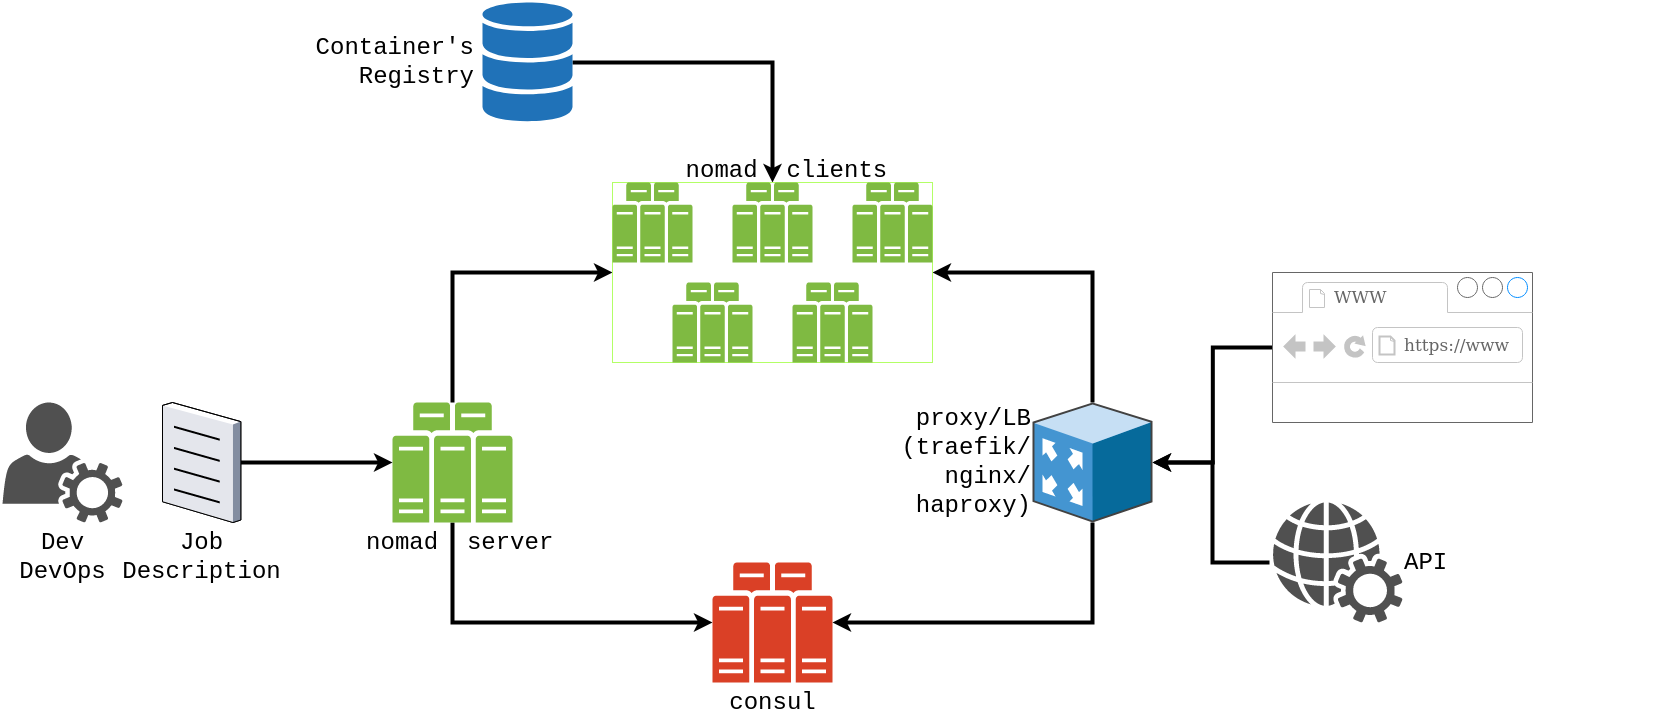
\includegraphics[width=\textwidth]{nomad-frame.png}
\caption{A service mesh based on nomad}
\label{fig:nomad}
\end{figure*}
\section{\texttt{pot}}\label{sec:pot}
In this section, we'll present \texttt{pot}~\cite{pot}, a generic jail management tool, similar to other jail related tools, based on FreeBSD technologies like \texttt{VNET(9)}, \texttt{zfs(8)}, \texttt{pf(4)} and \texttt{rctl(4)}. It evolved over time to also support the typical container carateristics, like, not persistent jails and not forking start commands.

In this paper, we will focus on the only model that has been developed to work as container, the \texttt{pot} of type single.
The single type \texttt{pot} is designed to contain the whole needed files in a single ZFS dataset, allowing to easily create snapshots and compressed images.

The \texttt{pot create} command will create a pot with the FreeBSD base system and all default settings.

The bootstrap/provision of a \texttt{pot} can be automated providing a bootstrap script called flavor to the create command.

When a pot is created and bootstrapped, an image can be generated via the \texttt{pot export} command. The image is a compressed snapshot of the entire file system representing the jail and of its configuration.

Symmetrically, a \texttt{pot} can be created from an image via the command \texttt{pot import}. Import uses \texttt{fetch(1)} to download a pot image, hence to host images a simple webserver can be used. Images are weakly protected by a skein hash, designed to detected transfer errors; however, the hash mechanism is not designed to detect tampering or other potential security breaches. A self-hosted registry is the suggested solution.

Additionally, \texttt{pot} suports four different networking model:
\begin{itemize}
	\item inherit (host): the jail inherit the host network stack
	\item alias: the jail has a unique IP applied as alias to the host network interface
	\item public-bridge: the jail is attached to a virtual network on a shared bridge interface. The bridge is connected to the host network interface using NAT
	\item private-bridge: the jail is attached to a virtual network on a private bridge, shared with few selected jails. The bridge is connected ot the host network interface using NAT
\end{itemize}

\texttt{pot} allows also to run jails with not forking commands. However, if that happens, the terminal used to start the jail will be held by the jail itself. \texttt{pot} start a jail using the \texttt{jail -c} command. However, because the starting command doesn't return, \texttt{pot} is taking care of applying resource limitation and not persistent attribute to the jail, if needed.

\section{consul, nomad and traefik}\label{sec:ServiceMesh}
In this section, we’ll present the service mesh we implemented using open-source cluster management software. The solution we used has three main components:
\begin{itemize}
	\item \texttt{consul}: a service discovery system, where network service can be registered and monitored~\cite{consul}
	\item \texttt{nomad}: a container orchestrator, where the deploy of services can be scheduled.\ nomad will take care of deploying container on available nodes and to automatically register the deployed services on consul~\cite{nomad}
	\item \texttt{traefik}: a layer 7 load balancer, that is able to route network traffic to the service registered in consul~\cite{traefik}
\end{itemize}

The typical deploy process, as illustrated in Fig.~\ref{fig:nomad} is the following:
\begin{itemize}
	\item a request to deploy a service (called ‘job’) is sent to nomad
	\item nomad will schedule the deploy and the execution of the service to a suitable node
	\item once the container is deployed and successfully started, the service is registered on consul
	\item consul will add the new service to its service catalog, where information to reach the service (like the IP address and the TCP port) are stored
	\item consul also start to check the health status of the service, to keep the list of healthy instances up to date
\end{itemize}

To make services easily reachable, an ingress point has to be configured. An ingress point is a layer 7 load balancer or proxy, that redirect network traffic to the services running on the nomad clients using the information provided by consul. An additional component, usually called sidecar, is responsible to keep the list of the services served by the proxy up to date.

As proxy, we used traefik that already support consul as service discovery provider, with no additional sidecar to be added or configured.

All those tools are already available on FreeBSD, as ports or as packages, so no additional effort to install and use them was needed.

However, nomad is the only tool that needd to be extended, in order to orchestrate containers built with \texttt{pot}; all the other tools are already well supported on FreeBSD and they don’t need any additional customization.

\begin{lstlisting}[float=*, backgroundcolor=\color{listing-bg},numbers=left,label=list:nomad,caption={An example of a nomad job}]
job "nginx-pot" {
  datacenters = ["minipot"]
  type = "service"
  group "group1" {
    count = 1 
    task "www" {
      driver = "pot"
      config {
        image = "https://pot-registry.zapto.org/registry/"
        pot = "FBSD121-nginx"
        tag = "1.2"
        command = "nginx -g 'daemon off;'"
        port_map = {
          http = "80"
        }
      }
      service {
        tags = ["pot", "www"]
        name = "hello-pot"
        port = "http"
         check {
            type     = "tcp"
            name     = "tcp"
            interval = "5s"
            timeout  = "2s"
          }
      }
      resources {
        cpu = 200
        memory = 64
        network {
          mbits = 10
          port "http" {}
        }
      }
    }
  }
}
\end{lstlisting}
\section{nomad pot driver}\label{sec:nomad-pot-driver}
As said in the previous section, nomad is the only tool that has been extended to support \texttt{pot} jails in the service mesh.

In particular, nomad is designed to support different types of containers, implementing a driver-based architecture. We developed a new nomad driver~\cite{nomad-pot-driver}, to add \texttt{pot} support to nomad.

When a ‘job’ based on \texttt{pot} is requested to nomad, the orchestrator will look for nomad clients that support the nomad-pot-driver.

We will use the example in Listing~\ref{list:nomad} to explain how to interact with nomad and the driver.

Every task represents a container. At line 7, we select the \texttt{pot} driver for the task \texttt{www}. At line 8, the \texttt{config} stanza provides further instructions to the driver, like
\begin{itemize}
	\item line 9: the base URL of the images
	\item line 10: the name of the image we want to use
	\item line 11: the tag, used to version images
	\item line 12: the jail initial command
\end{itemize}
By default, the driver will use the public-bridge network type.

At line 10, the service stanza is used to configure what services has to be registered. In particular:
\begin{itemize}
	\item line 19: the name of the service
	\item line 18: tags like arbitrary labels, and they can be used to filter searches in consul
	\item line 21: the check that consul will run to monitor the health status of the service
\end{itemize}

\subsection{Automatic port exposure}
The service we are running is a \texttt{nginx} web server, listening on port 80. However, only one process can listen on port 80 at a time, limiting the number of containers allowed to run.

To overcome this heavy limitation, nomad allocate a different TCP port, computed when the container is deployed, and then interact with \texttt{pot} to automatically insert a redirection rule to expose the service running inside the container to the ouside.

You can see in the Listing~\ref{list:nomad} how this is achieved:
\begin{itemize}
	\item line 33: a resource of type port is decleared: the name ``http'' is arbitrary
	\item line 14: tell nomad, and then the driver, that the port ``http'' has to be mapped to port 80; \texttt{pot} will automatically insert a redirection rule to forward the traffic from port ``http'' to the port 80 of the container
	\item line 20: nomad will register in consul that the service is reachable at port ``http''
\end{itemize}
The port ``http'' is used as placeholder inside the job description file; when nomad deploys the service, it will allocate a real port number that will be used instead of the ``http'' placeholder.

\section{\texttt{pot} images}\label{sec:Images}
A direct consequence of a service mesh is the clear separation between the system that created the container image and the system where the image is deployed.

As described in Section~\ref{sec:pot}, the steps to create a \texttt{pot} image are:
\begin{itemize}
	\item create a \texttt{pot}
	\item bootstrap/provision the container
		\subitem install packages
		\subitem create directories and/or files
		\subitem create or modify configuration files
	\item take a snapshot of the provisioned image
	\item export the snapshot to a compressed file
\end{itemize}

All those steps are already supported by \texttt{pot}. To further improve process automation, the provision steps can be automated with shell scripts that can be automatically executed when the \texttt{pot} is created.

However, the technologies used to implement \texttt{pot} are FreeBSD specific. Even if other operating systems provide similar technologies, \texttt{jail(8)} is still very FreeBSD specific. That means that \texttt{pot} can only be used on a FreeBSD system.

To remove this constraint, a new tool name \texttt{potMachine}~\cite{potMachine} has been developed. \texttt{potMachine} allows developer to create and execute \texttt{pot} images on different operating systems. To executed FreeBSD binaries on different systems, \texttt{potMachine} creates a virtal machine running FreeBSD and will forward all commands to this VM.

\section{Conclusion}\label{sec:Conclusion}
We showed how FreeBSD can be used to create its own container model, similar to Docker, using FreeBSD technologies like \texttt{jail(8)}, \texttt{VNET(9)}, \texttt{zfs(8)}, \texttt{pf(4)} and \texttt{rctl(4)}.

Moreover, no operating system features have been added to achieve this goal. A bit of automation has been added and few utilities have been written to simplify the workflow, but nothing else.

Finally we integrated the container model in a service mesh, a typical cloud computing architecture, and validated the model.

We showed that it’s possible to separate the jail image creation and the image deploy.
All the code is open source, and available in the ports tree or as package, ready to be installed in any FreeBSD system.

\begin{thebibliography}{1}

\bibitem{jail}
	Poul-Henning Kamp and Robert N. M. Watson, \emph{ Jails: Confining the omnipotent root}, 2nd Intl. SANE Conference, 2000.
\bibitem{pot}
	\emph{https://github.com/pizzamig/pot}
\bibitem{nomad-pot-driver}
	\emph{https://github.com/trivago/nomad-pot-driver}
\bibitem{potMachine}
	\emph{https://github.com/ebarriosjr/potMachine}
\bibitem{nomad}
	\emph{https://www.nomadproject.io}
\bibitem{consul}
	\emph{https://www.consul.io}
\bibitem{traefik}
	\emph{https://docs.traefik.io}
\bibitem{docker}
	\emph{https://www.docker.com}
\end{thebibliography}

\end{document}

